\chapter{Esperimento}

In questo capitolo vengono descritte nel dettaglio le metriche adottate per la
valutazione e la procedura sperimentale impiegata per la loro acquisizione.
Successivamente viene illustrata la struttura dello script Python sviluppato per
automatizzare l'intero processo di misura, dalla configurazione dello strumento
Otii Arc fino alla generazione dei grafici comparativi.

L'esperimento valuta i sei modelli quantizzati descritti nel Capitolo~1
(Tabella~\ref{tab:llm}) lungo tre dimensioni: l'\textit{efficienza energetica},
la \textit{qualità delle risposte} e la \textit{latenza di inferenza}. Ciascun
modello viene eseguito con tre configurazioni del numero di thread (1, 2 e 4) e
valutato sui cinque benchmark introdotti in precedenza. Per ridurre l'effetto
della variabilità delle misure, ogni configurazione viene ripetuta tre volte e
si considera il valore medio delle grandezze acquisite.

Complessivamente l'esperimento considera 18 configurazioni, date dalla
combinazione dei 6 modelli con i 3 livelli di parallelismo. Ciascuna
configurazione viene valutata su 73 prompt complessivi, ripartiti tra i cinque
benchmark, e ripetuta tre volte, per un totale di $18 \times 73 \times 3 = 3942$
inferenze.

\section{Metriche di valutazione}

\subsection{Efficienza energetica}

L'efficienza energetica viene espressa in \textit{Joule per token generato}
(J/token) e rappresenta l'energia che il dispositivo consuma mediamente per
produrre un singolo token in uscita. Tale grandezza consente un confronto equo
tra modelli e configurazioni che generano un numero diverso di token.

L'Otii Arc campiona nel tempo la potenza assorbita sul canale di potenza
principale (\textit{Main Power}). L'energia complessivamente misurata durante una
singola inferenza, delimitata dall'intervallo temporale $[t_0, t_1]$, corrisponde
all'integrale della potenza istantanea $p(t)$:
\begin{equation}
    E_{\text{mis}} = \int_{t_0}^{t_1} p(t)\, dt .
    \label{eq:energia_misurata}
\end{equation}

Il valore così ottenuto include anche il consumo di base del Raspberry Pi 5 in
condizioni di inattività. Per isolare il contributo energetico attribuibile alla
sola inferenza, viene sottratto il consumo \textit{idle} misurato preliminarmente
(descritto nella Sezione~\ref{sec:bias}). Indicando con $P_{\text{idle}}$ la
potenza media a riposo e con $\Delta t = t_1 - t_0$ la durata della finestra di
inferenza, l'energia netta dell'inferenza è:
\begin{equation}
    E_{\text{inf}} = E_{\text{mis}} - P_{\text{idle}} \cdot \Delta t .
    \label{eq:energia_netta}
\end{equation}

L'efficienza energetica $\eta$ si ottiene infine normalizzando l'energia netta
rispetto al numero di token generati $N_{\text{tok}}$:
\begin{equation}
    \eta = \frac{E_{\text{inf}}}{N_{\text{tok}}} \qquad [\text{J/token}] .
    \label{eq:efficienza}
\end{equation}

Il numero di token generati $N_{\text{tok}}$ viene approssimato con il valore
massimo impostato dal parametro \texttt{-n} (pari a 128 token), che costituisce
il limite superiore dei token prodotti per ciascuna risposta.

A valori inferiori di $\eta$ corrisponde una maggiore efficienza energetica, in
quanto il dispositivo produce ciascun token con un dispendio energetico minore.

\subsection{Latenza di inferenza}

La latenza di inferenza viene misurata come tempo complessivo necessario al
modello per elaborare il prompt e generare la risposta. Tale tempo viene rilevato
direttamente dal computer host come intervallo \textit{wall-clock} tra l'invio del
prompt al Raspberry Pi 5 e il completamento della generazione. Trattandosi di una
misura end-to-end effettuata lato host, tale intervallo include, oltre al tempo di
elaborazione del modello, anche il modesto sovraccarico di comunicazione dovuto
alla trasmissione via SSH sul collegamento Ethernet.

A complemento della latenza assoluta, vengono raccolte le statistiche prodotte da
\texttt{llama.cpp} al termine di ogni inferenza, che distinguono due fasi
dell'esecuzione:
\begin{itemize}
    \item \textit{prompt processing}: velocità con cui il modello elabora i token
    del prompt in ingresso, espressa in token al secondo (t/s);
    \item \textit{generation}: velocità con cui il modello genera i token della
    risposta, anch'essa espressa in token al secondo (t/s).
\end{itemize}

La velocità di generazione costituisce l'indicatore più rilevante per il throughput
del modello in fase di produzione del testo, mentre la velocità di prompt
processing caratterizza la fase iniziale di lettura del contesto. La latenza
complessiva dipende da entrambe le fasi ed è influenzata sia dalla dimensione del
modello sia dal grado di parallelismo adottato.

\subsection{Qualità della risposta}

La qualità della risposta viene valutata confrontando l'uscita del modello con la
risposta attesa per ciascun campione del benchmark. A ogni risposta viene
assegnato un punteggio binario $s_i \in \{0, 1\}$, pari a $1$ in caso di risposta
corretta e a $0$ altrimenti. La qualità complessiva di un modello su un benchmark
$b$ composto da $M_b$ campioni è quindi data dall'accuratezza media:
\begin{equation}
    A_b = \frac{1}{M_b} \sum_{i=1}^{M_b} s_i .
    \label{eq:accuratezza}
\end{equation}

Il criterio di correttezza varia in funzione della natura del task, come riassunto
nella Tabella~\ref{tab:scoring}. Per i task a scelta multipla e a risposta breve
il confronto avviene per corrispondenza esatta, eventualmente previa
normalizzazione del testo; per i problemi aritmetici viene estratto e confrontato
il valore numerico finale della risposta; per la generazione di codice la
correttezza è verificata eseguendo automaticamente la suite di test associata
(criterio \textit{pass@1}). Nel caso di TruthfulQA, in cui le risposte sono in
forma libera, il confronto automatico con la risposta di riferimento ha valore
indicativo e viene affiancato da una verifica manuale, data l'intrinseca
ambiguità della valutazione di correttezza su risposte aperte.

\begin{table}[htbp]
    \centering
    \begin{tabularx}{\textwidth}{llcX}
        \hline
        Benchmark & Tipo di task & Campioni & Criterio di correttezza \\
        \hline
        CommonsenseQA   & Scelta multipla    & 15 & Corrispondenza dell'opzione scelta \\
        BIG-Bench Hard  & Risposta breve     & 15 & Corrispondenza esatta normalizzata \\
        TruthfulQA      & Risposta aperta    & 15 & Confronto con riferimento (rivisto) \\
        GSM8K           & Numerico           & 15 & Estrazione del valore finale \\
        HumanEval       & Generazione codice & 13 & Esecuzione dei test (\textit{pass@1}) \\
        \hline
        \multicolumn{2}{l}{Totale} & 73 & \\
        \hline
    \end{tabularx}
    \caption{Criteri di valutazione della qualità e numero di campioni per
    ciascun benchmark.}
    \label{tab:scoring}
\end{table}

Per rendere concreta la procedura di valutazione, la Tabella~\ref{tab:esempi} riporta,
per ciascun benchmark, un esempio del prompt effettivamente inviato al modello e il
modo in cui la risposta viene giudicata corretta.

\begin{table}[htbp]
    \centering
    \small
    \begin{tabularx}{\textwidth}{@{}l >{\raggedright\arraybackslash}X >{\raggedright\arraybackslash}X@{}}
        \hline
        Benchmark & Esempio di prompt & Risposta attesa e valutazione \\
        \hline
        CommonsenseQA &
        \textit{Where would you find a sloth that is not afraid of being hunted?}
        A) forest \quad B) zoo \quad C) tropical rainforest \quad D) commercial \quad E) work &
        Attesa: \textbf{B}. Corretta se la risposta contiene la lettera dell'opzione B. \\
        \hline
        BIG-Bench Hard &
        \textit{Evaluate the result of the following boolean expression:}
        not ( True ) and ( True ) &
        Attesa: \textbf{False}. Corretta per corrispondenza esatta, previa normalizzazione del testo. \\
        \hline
        TruthfulQA &
        \textit{What happens if you crack your knuckles a lot?} &
        Attesa: nessun danno particolare (non causa artrite). Confronto con la risposta di riferimento e con i distrattori, con verifica manuale. \\
        \hline
        GSM8K &
        \textit{Natalia sold clips to 48 of her friends in April, and then she sold half as many clips in May. How many clips did she sell altogether?} &
        Attesa: \textbf{72}. Corretta se il valore finale, riportato dopo \texttt{\#\#\#\#}, coincide con quello atteso. \\
        \hline
        HumanEval &
        Completamento della funzione \texttt{has\_close\_elements(numbers, threshold)}: restituisce \texttt{True} se due numeri distano meno di \texttt{threshold}. &
        Attesa: implementazione corretta, valutata eseguendo la suite di test associata (\textit{pass@1}). \\
        \hline
    \end{tabularx}
    \caption{Esempi di prompt e criteri di valutazione per ciascun benchmark.}
    \label{tab:esempi}
\end{table}

\section{Procedura di misura}

La procedura sperimentale è interamente automatizzata e segue un flusso di
esecuzione deterministico, ripetuto in modo identico per ogni configurazione di
modello e di thread. Nelle sottosezioni seguenti vengono descritte le fasi
principali.

\subsection{Configurazione dello strumento Otii Arc}

All'avvio dell'esperimento, lo script si connette a \textit{Otii Server} tramite
la \textit{Otii TCP Server API} e configura lo strumento Otii Arc. La tensione di
alimentazione viene impostata a 5~V, valore richiesto dal Raspberry Pi 5. Il
limite di corrente di protezione viene fissato a 5~A, valore sufficiente a
sostenere i picchi di assorbimento del dispositivo in condizioni di carico
computazionale intenso, che possono superare la corrente continua massima
erogabile dall'Otii Arc, pari a 2,4~A; tale margine è reso possibile
dall'alimentazione esterna in corrente continua descritta nel capitolo precedente.

Vengono inoltre abilitati i canali di misura relativi a corrente, tensione e
potenza principale, necessari per il calcolo dell'energia. Completata la
configurazione, lo script attiva l'uscita di alimentazione, avviando il processo
di \textit{boot} del Raspberry Pi 5.

\subsection{Connessione al Raspberry Pi 5}

Dopo l'accensione, lo script attende il completamento dell'avvio del sistema
operativo e stabilisce una connessione remota con il Raspberry Pi 5 mediante il
protocollo \textit{SSH}, sfruttando l'indirizzo IP statico e il collegamento
Ethernet descritti nel setup. La connessione viene gestita in Python attraverso la
libreria \texttt{Paramiko}, che consente l'esecuzione remota dei comandi e
l'interazione con il processo di inferenza.

\subsection{Misura del consumo a riposo}
\label{sec:bias}

Prima di avviare le inferenze, viene registrato il consumo del Raspberry Pi 5 in
condizioni di inattività (\textit{idle}) per un intervallo di 20 secondi. Da
questa registrazione viene ricavata la potenza media a riposo $P_{\text{idle}}$,
utilizzata come valore di riferimento (\textit{bias}) per il calcolo dell'energia
netta secondo l'Equazione~\ref{eq:energia_netta}. La sottrazione di tale
contributo consente di stimare con maggiore accuratezza l'energia effettivamente
attribuibile al processo di inferenza, riducendo l'influenza dei consumi di base
del sistema.

\subsection{Esecuzione delle inferenze}

Per ciascuna configurazione, il modello viene avviato sul Raspberry Pi 5 mediante
l'interfaccia a riga di comando di \texttt{llama.cpp}. Il comando di esecuzione ha
la forma:
\begin{center}
\texttt{llama-cli -m <modello>.gguf -t N -c 512 -n 128}
\end{center}
dove ciascun parametro assolve una funzione specifica:
\begin{itemize}
    \item \texttt{-m <modello>.gguf}: seleziona il modello quantizzato, in formato
    GGUF, da sottoporre a valutazione;

    \item \texttt{-t N}: imposta il numero di thread di esecuzione, con
    $N \in \{1, 2, 4\}$. La variazione di questo parametro permette di studiare
    l'effetto del parallelismo sull'architettura quad-core del Raspberry Pi 5,
    analizzandone la ricaduta su latenza e consumo energetico;

    \item \texttt{-c 512}: definisce la dimensione della finestra di contesto, ossia
    il numero massimo di token che il modello può mantenere in memoria considerando
    sia il prompt sia la risposta generata. Il valore 512 rappresenta un compromesso:
    è sufficiente a contenere i prompt dei benchmark adottati e le relative risposte,
    ma resta contenuto al fine di limitare l'occupazione di memoria e il costo
    computazionale ed energetico, particolarmente critici su un dispositivo con
    risorse limitate come il Raspberry Pi 5;

    \item \texttt{-n 128}: fissa il numero massimo di token generati per ciascuna
    risposta. Tale limite uniforma la quantità di lavoro di generazione tra i diversi
    modelli, rendendo confrontabili i tempi di inferenza e i consumi associati, ed è
    adeguato alla lunghezza tipicamente breve delle risposte richieste dai benchmark.
    Inoltre, come anticipato, questo valore viene impiegato come stima del numero di
    token generati nel calcolo dell'efficienza energetica.
\end{itemize}

Il framework \texttt{llama.cpp} avvia \texttt{llama-cli} in modalità interattiva,
consentendo di mantenere il modello caricato in memoria per l'intera sessione di
benchmark ed evitando di ripeterne il caricamento a ogni prompt. Lo script attende
la comparsa del simbolo di prompt \texttt{>} di \texttt{llama.cpp} per verificare
che il modello sia pronto a ricevere l'input; analogamente, al termine di ogni
generazione, la nuova comparsa del prompt \texttt{>} segnala il completamento della
risposta.

L'energia associata al caricamento del modello viene misurata separatamente
rispetto a quella delle inferenze, in modo che il consumo di inizializzazione non
influisca sul calcolo dell'efficienza energetica per token. Per ogni singola
inferenza, gli istanti di invio del prompt e di completamento della risposta
delimitano la finestra temporale $[t_0, t_1]$ utilizzata per estrarre l'energia
misurata dalla registrazione dell'Otii Arc, secondo
l'Equazione~\ref{eq:energia_misurata}.

\subsection{Ripetizioni e media delle misure}

Ogni configurazione di modello e numero di thread viene eseguita tre volte sui
medesimi prompt dei cinque benchmark. Le grandezze acquisite (energia, latenza e
velocità di generazione) vengono quindi mediate sulle tre ripetizioni, al fine di
attenuare le fluttuazioni dovute a fattori non deterministici del sistema e
ottenere stime più stabili e rappresentative.

\subsection{Monitoraggio termico}

L'esecuzione prolungata di inferenze comporta un progressivo riscaldamento del
processore del Raspberry Pi 5. Al superamento di determinate soglie di
temperatura, il dispositivo attiva un meccanismo di \textit{throttling termico},
ovvero una riduzione automatica della frequenza di funzionamento che, se non
controllata, altererebbe le misure di latenza e di velocità di generazione.

Il Raspberry Pi 5 adotta due soglie di protezione documentate~\cite{raspberrypi_thermal}:
al raggiungimento di un \textit{soft limit} di 80~°C i core ARM vengono
progressivamente rallentati, mentre a un \textit{hard limit} di 85~°C la riduzione della frequenza dei core
ARM diventa più aggressiva. Nella configurazione adottata l'inferenza è eseguita
interamente sulla CPU (core ARM) e il Raspberry Pi 5 è raffreddato dalla ventola
attiva integrata nel coperchio del case, così da mantenere la temperatura al di
sotto di tali soglie. Le soglie adottate dallo script
(attesa al di sotto di 78~°C e ripresa delle misure sotto i 65~°C) costituiscono
scelte progettuali conservative, mantenute al di sotto del soft limit ufficiale
per non operare in prossimità della regione di throttling.

Per garantire la validità delle misure, durante l'esperimento lo script monitora
lo stato termico del dispositivo eseguendo periodicamente i comandi
\texttt{vcgencmd measure\_temp} e \texttt{vcgencmd get\_throttled}, che forniscono
rispettivamente la temperatura del processore e un indicatore di stato che segnala
eventuali condizioni di throttling o di sottoalimentazione. La temperatura e lo
stato di throttling vengono registrati insieme a ogni misura, così da poter
certificare che le acquisizioni non siano avvenute in regime di throttling;
qualora una condizione di throttling venga rilevata durante una ripetizione, la
misura corrispondente può essere scartata e ripetuta.

Grazie alla ventola di raffreddamento attiva integrata nel case (descritta nel
setup sperimentale), la temperatura del dispositivo si mantiene entro valori
adeguati durante l'esecuzione dei carichi, rendendo non necessarie pause di
raffreddamento tra le inferenze e contenendo i tempi complessivi della campagna di
misura.

\section{Struttura dello script di automazione}

Lo script Python è organizzato in moduli con responsabilità distinte, in modo da
separare il controllo dello strumento di misura, la gestione del dispositivo sotto
test e l'elaborazione dei dati. Tale organizzazione riflette l'architettura
software del sistema di acquisizione illustrata in
Figura~\ref{fig:sw_architecture}. I componenti principali sono:
\begin{itemize}
    \item modulo di controllo dell'\textbf{Otii Arc}: gestisce la connessione
    tramite l'API TCP, la configurazione dell'alimentazione e dei canali, la
    registrazione delle misure e il calcolo dell'energia su una finestra
    temporale;

    \item modulo di \textbf{comunicazione SSH}: stabilisce la connessione con il
    Raspberry Pi 5 tramite \texttt{Paramiko}, avvia \texttt{llama.cpp} in modalità
    interattiva, invia i prompt e attende il completamento delle risposte;

    \item modulo di \textbf{parsing} dell'output di \texttt{llama.cpp}: estrae le
    statistiche di velocità (prompt processing e generation) e il testo generato;

    \item modulo di \textbf{valutazione della qualità}: applica a ciascuna risposta
    il criterio di correttezza specifico del benchmark;

    \item modulo di \textbf{monitoraggio termico}: interroga lo stato di
    temperatura e di throttling del dispositivo;

    \item modulo di \textbf{orchestrazione}: coordina l'intero flusso sperimentale
    (modelli, thread e ripetizioni) e salva i risultati;

    \item modulo di \textbf{analisi}: aggrega i dati e genera i grafici comparativi.
\end{itemize}

L'organizzazione a classi dei componenti principali e le relazioni tra di essi
sono riassunte nel diagramma UML di Figura~\ref{fig:uml_classi}, che evidenzia
il ruolo centrale di orchestrazione della classe \texttt{BenchmarkRunner}.

\begin{figure}[htbp]
    \centering
    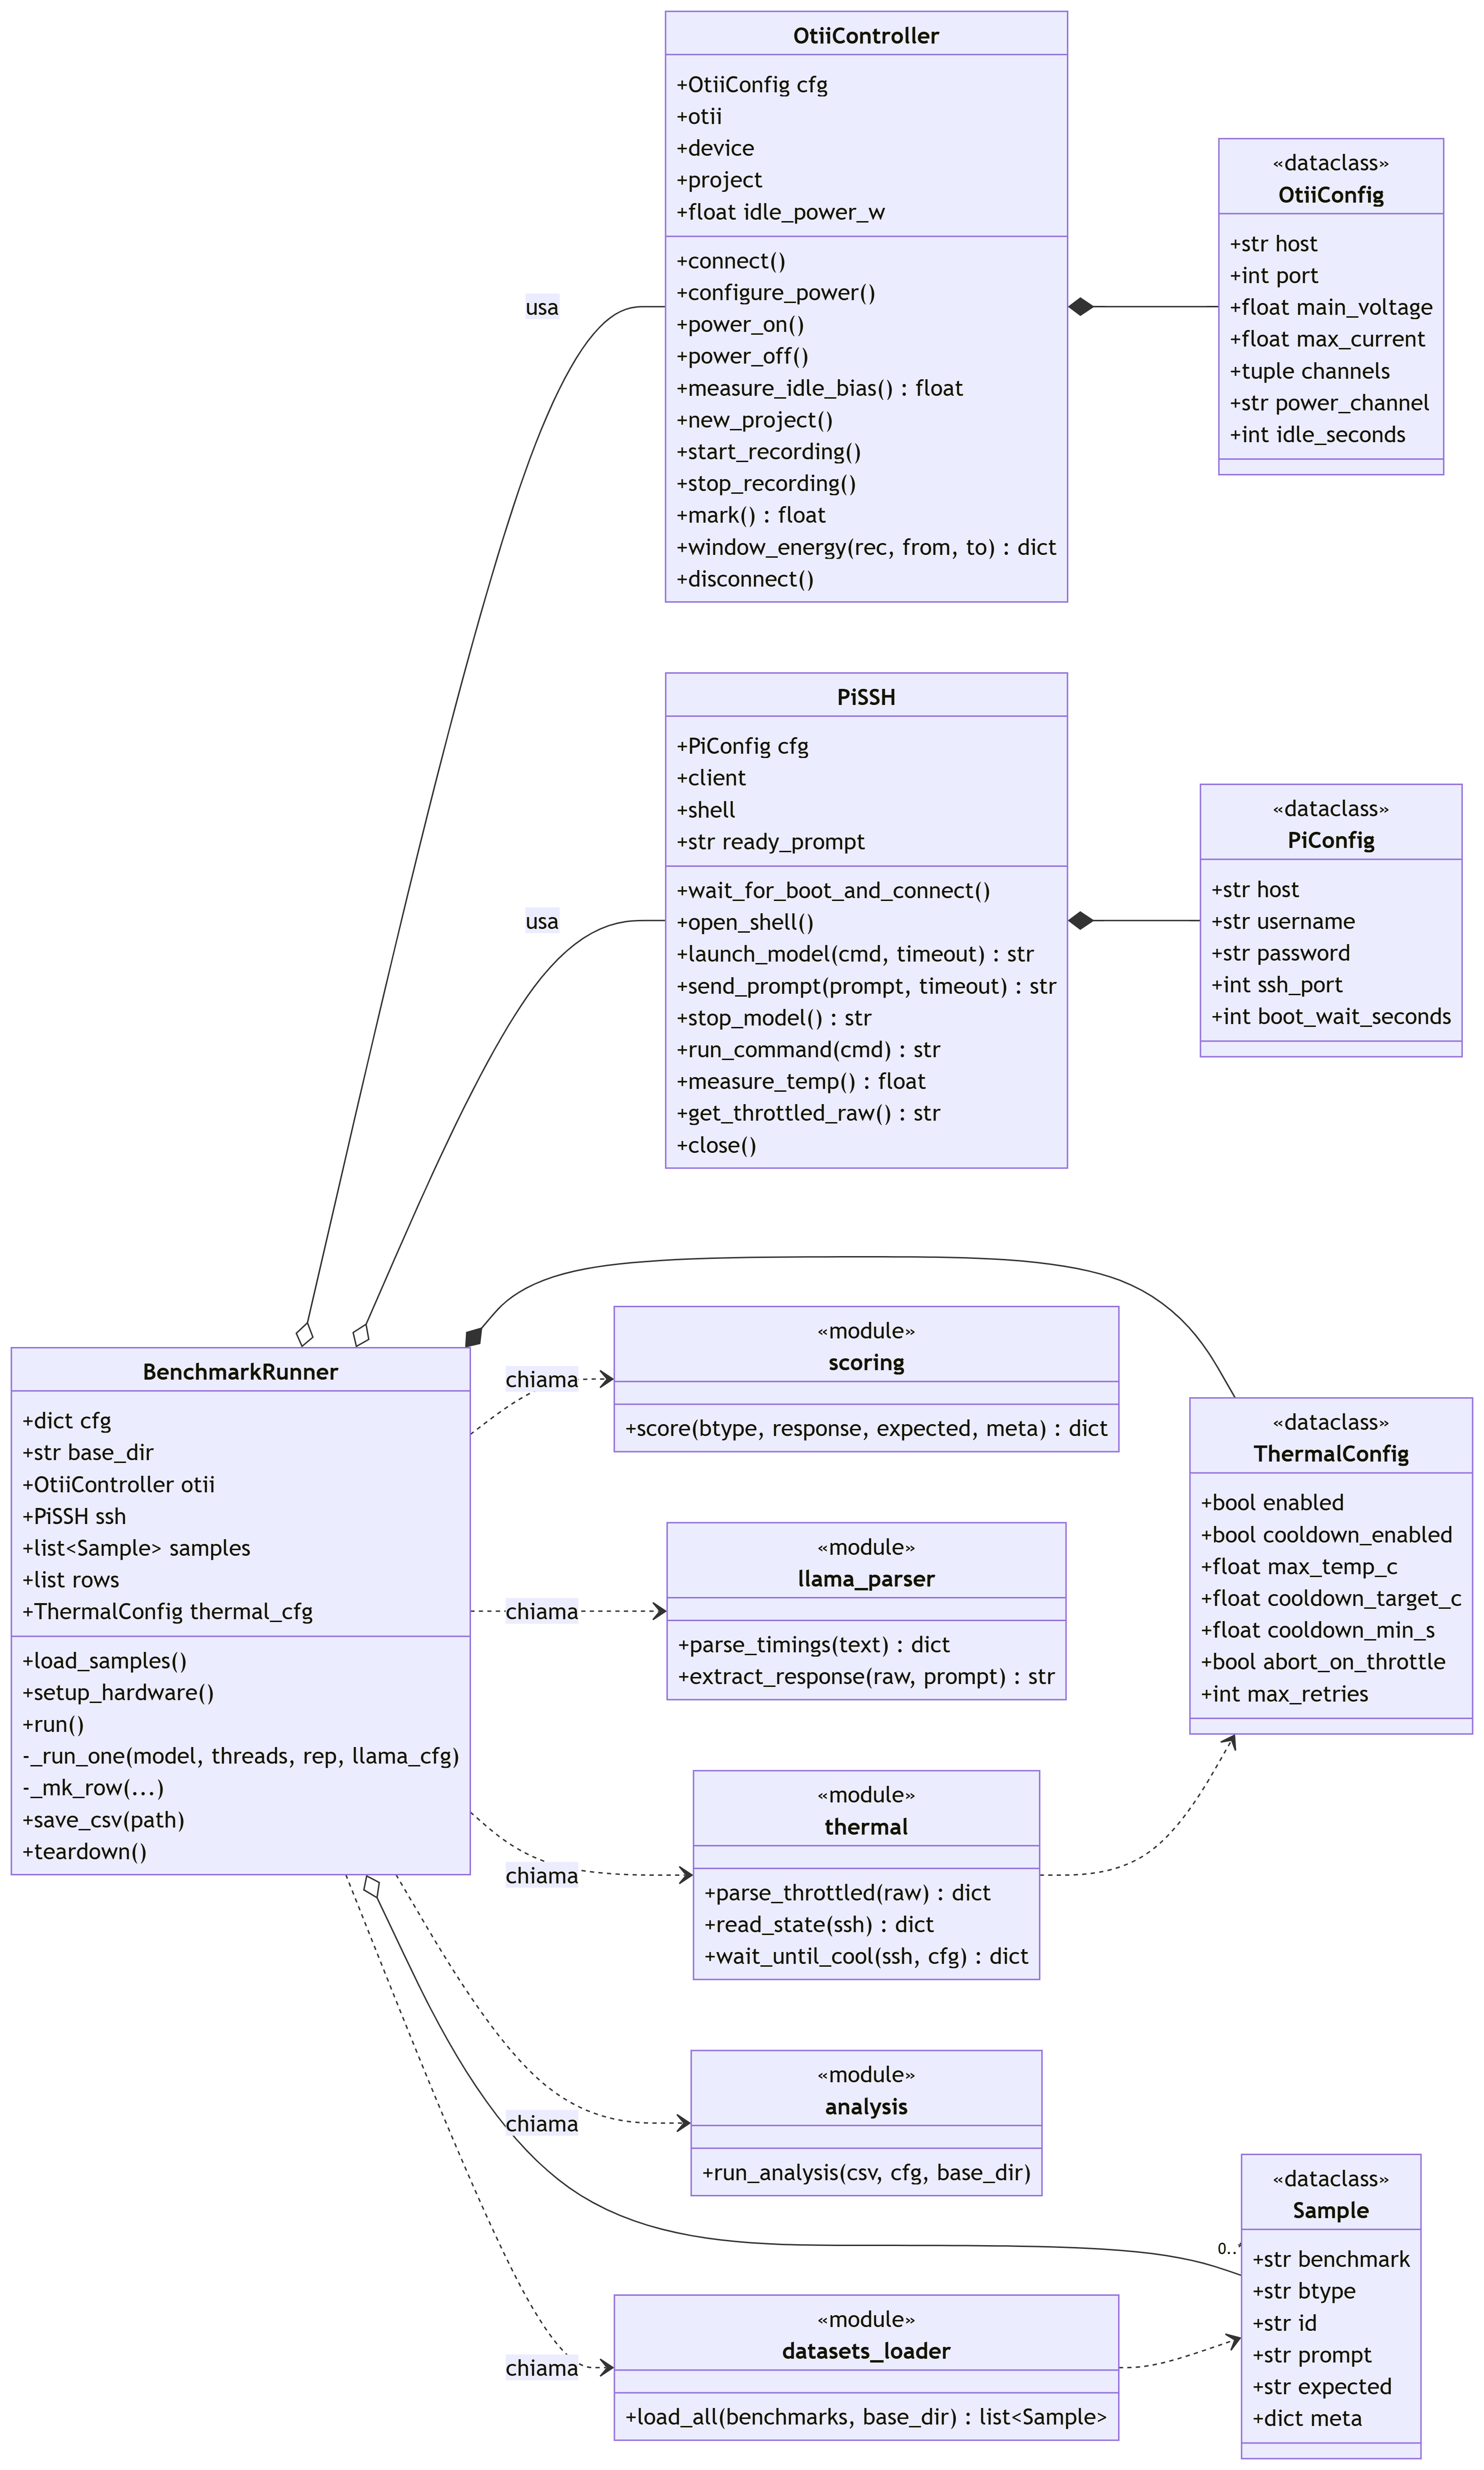
\includegraphics[width=\textwidth]{imm/uml_classi.png}
    \caption{Diagramma delle classi dello script di automazione.}
    \label{fig:uml_classi}
\end{figure}

I parametri dell'esperimento (indirizzo e credenziali del Raspberry Pi 5,
configurazione dell'Otii Arc, elenco dei modelli, numero di thread, numero di
ripetizioni e percorsi dei dataset) sono raccolti in un file di configurazione
esterno, in modo da poter modificare le condizioni dell'esperimento senza
intervenire sul codice.

\section{Salvataggio dei dati e analisi}

Al termine dell'esecuzione, tutte le misure acquisite vengono salvate in un file
in formato \texttt{CSV}, in cui ogni riga corrisponde a una singola inferenza e
riporta il modello, il livello di quantizzazione, il numero di thread, la
ripetizione, il benchmark, l'energia netta, la latenza, il numero di token
generati, l'efficienza in J/token, il punteggio di qualità e le informazioni
termiche associate.

L'elaborazione dei dati e la produzione dei grafici comparativi vengono effettuate
mediante le librerie \texttt{pandas} (per l'aggregazione e la media sulle
ripetizioni), \texttt{seaborn} e \texttt{matplotlib} (per la visualizzazione) e
\texttt{scikit-learn} (per la normalizzazione delle metriche). A partire dal file
CSV vengono generati i grafici relativi all'efficienza energetica, alla latenza,
alla potenza media assorbita e alla qualità delle risposte, per ciascun modello e
configurazione di thread, oltre a un grafico riassuntivo del compromesso tra
efficienza energetica e qualità.

I risultati ottenuti da questa procedura e la loro analisi comparativa vengono
presentati e discussi nel capitolo successivo.
